\documentclass[11pt]{report}	
\usepackage[ngerman]{babel}
\usepackage{subscript}
\usepackage{hyperref}
\usepackage{graphicx}
\usepackage{float}
\usepackage{multirow}

\newenvironment{mylisting}
{\begin{list}{}{\setlength{\leftmargin}{1em}}\item\scriptsize\bfseries}
{\end{list}}

\begin{document}
\begin{titlepage}
\title{Satellit - Raketen - Problem}
\begin{figure}[t]
\centering
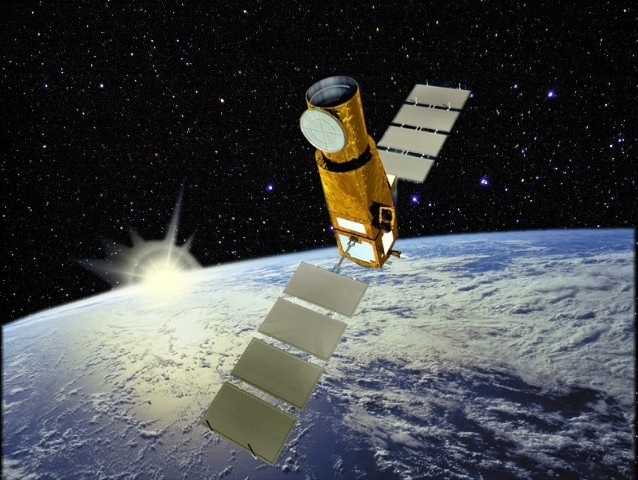
\includegraphics{corot-Ausschnitt-klein.jpg}
%\caption{Titelbild}
\label{title}
\end{figure}
\author{Gennaro Piano \\ Philipp Schalcher}
\date{\today}
\maketitle
\end{titlepage}
	
\tableofcontents
\newpage

\chapter{Einleitung}
Auftrag ist es, eine Simulation eines Raketenstarts und –flugs zu bauen. Die Rakete wird mit einer bestimmten F"ullmenge eines Treibstoffes von einem Punkt auf der Erde starten. Das Programm soll aus den angegebenen Parametern eine Flugbahn berechnen, welche die folgenden Bedingungen erf"ullt:
	
\begin{itemize}
\item Rakete kommt mit dem Treibstoff in den Orbit des Satelliten.
\item Rakete ist am Ende des Fluges beim Satelliten angedockt und der Treibstoff ist verbraucht.
\item Rakete und Satellit haben am Ende die gleiche Geschwindigkeit.
\end{itemize}
\section{Erde}
Die Erde befindet sich im Zentrum des 				Systems. Sie hat eine definierte Masse und 			eine definierte Gravitation. Beide sind 				konstant.
\section{Satellit}
Der Satellit befindet sich zum Startzeitpunkt in 	einer Umlaufbahn um die Erde. Er kreist in 			einer elliptischen Bewegung um die Erde. Wie die 	Erde ist dem Satellit eine definierte Masse 			zugewiesen. Ausserdem werden noch die 				Geschwindigkeit und die Position ben"otigt.
\section{Rakete}
Die Rakete steht zu Beginn an der Abschussrampe 		auf der Erde. Ihr ist ebenfalls eine Masse 			zugewiesen. Dazu kommen noch Treibstoffmenge 		(variabel), Verbrennungsgrad des Treibstoffes 		(variabel) und Position auf der Erde. Das 			Programm soll nun Geschwindigkeit, Richtung und 		Abschusszeitpunkt berechnen. Die Rakete wird 		dann diesen Weg abfliegen und so zum Satelliten 		gelangen, an welchem sie dann andocken wird.
\section{Abgrenzungen}
Die K"orper sollen physikalisch korrekt zu 			einander reagieren und Effekte wie 					Massenanziehung beinhalten. Allerdings werden 		"ausseren Einfl"usse ausgeschaltet. Sprich die 		Sonne und sonstige "ahnliche Einfl"usse werden 		ignoriert.
		
\newpage
		
\chapter{Mathematische Beziehung}
In diesem Abschnitt m"ochten wir mehr auf die 		mathematische Seite des Projektes eingehen. Dabei 	wird es in Satellit und Rakete unterteilt. Beide 	m"ussen bestimmte Voraussetzungen erf"ullen, damit das 	Programm am Schluss die korrekte Flugbahn berechnen kann.
		
\section{Satellit}
Der Satellit bewegt sich in einer elliptischen 		Bahn um die Erde. 
\begin{figure}[h!]
\centering
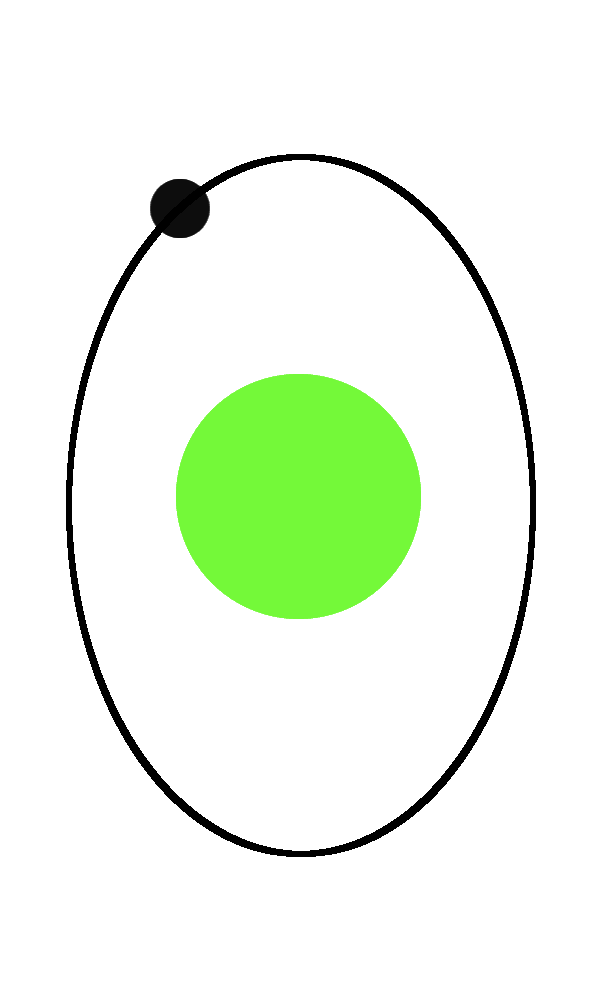
\includegraphics[width=4cm]{Erde_Umlaufbahn.png}
\caption{Erde mit Satellit in der Umlaufbahn}
\label{fig1}
\end{figure}
Diese Bahn wird haupts"achlich 	von der Startgeschwindigkeit und der 	Massenanziehungskraft der beiden K"orper 	verursacht.

Zum Zeitpunkt der Ausgangssituation kennen wir 		die Formel f"ur die Berechnung der Bahn nicht. 		Daher muss die Ellipse angen"ahert werden. Diese 		bewerkstelligen wir mit einem Polygon. Wir 			werden das Polygon durch die numerische 				Integration nach Euler erhalten.
		
\subsection{Euler-Theorie}
Die Integration nach Euler n"ahert einen 			Funktionsgraphen, wie schon erw"ahnt, durch 		ein Polygon an. Ein Polygon ist ein K"orper, 			welcher aus vielen verschiedenen 					Datenpunkten besteht. Diese sind mit einer 			Geraden verbunden. Daraus folgt, je mehr 			Unterteilungen wir durchf"uhren, desto 				genauer trifft das Ann"aherungspolygon den 			Funktionsgraphen. Allerdings brauchen wir 			f"ur die Euler-Berechnung noch die 					Beschleunigung des Satelliten zur Zeit t.
Der „0-Punkt“ (Punkt zur Zeit t = 0) kann 			durch einen Vektor in der Form (x\textsubscript{sat}, y\textsubscript{sat}, vx\textsubscript{sat}, vy\textsubscript{sat}). Dieser Vektor beschreibt 		die X- und die Y-Koordinate und die 						Geschwindigkeit v in X- und Y-Richtung. F"ur 			die Berechnung des neuen Punktes ben"otigen 			wir allerdings die Beschleunigung.
Wenn wir nun den Vektor ableiten werden die 			Positionskoordinaten zu den 							Geschwindigkeiten in die jeweilige 					Richtung. Sprich der Vektor sieht danach so aus:
\newline

\centering Satellit‘ = (vx\textsubscript{sat}, vy\textsubscript{sat}, ax\textsubscript{sat}, ay\textsubscript{sat})

\flushleft Wir sehen, dass die Geschwindigkeiten des Satelliten zur Beschleunigung werden. Die Beschleunigung k"onnen wir durch die Formel:

\begin{equation}
a_{x-Sat} = \frac{-g * m * (x_{Erde} - x_{Sat})}{|u|^3}
\end{equation}
\begin{equation}
a_{y-Sat} = \frac{-g * m * (y_{Erde} - y_{Sat})}{|u|^3}
\end{equation}
Nun haben wir die Informationen f"ur Euler durch differenzieren erhalten.
\linebreak

Euler integriert nun immer den Graphen "uber eine bestimmte Strecke (t\textsubscript{0} bis t\textsubscript{Ende}) in n Teilschritten. Die Anzahl der Teilschritte bekommen wir, wenn wir unser h (Unterschied zwischen t\textsubscript{0} und t1, t1 und t2, usw.) zuerst definieren, dann n berechnen durch (b-a)/h, dieses Ergebnis mathematisch korrekt runden (da n nur eine Ganze Zahl sein kann) und mit diesem n nochmals das korrekte h mit (b-a)/n ausrechnen.
Nun k"onnen wir unseren neuen Punkt des Satelliten ausrechen.  Den erhalten wir durch die folgende Gleichung:

\begin{equation}
Satellit_{neu} = Satellit_{alt} + h * Satellit_{alt}‘
\end{equation}
Sobald diese Rechnung durchgef"uhrt wurde, wird t um h erh"oht.
\linebreak

Da der Mensch diese kleinen Unterschiede bei der Darstellung gar nicht wahrnehmen k"onnte, wird der Satellit nur f"ur ein klar unterscheidbares t (bis jetzt t\textsubscript{0} + 0.1) neu gezeichnet. Somit entsteht die korrekte Flugbahn.
\newpage
\subsection{Wichtige Codestellen}
\subsubsection{Calculation.java}

\begin{mylisting}
\begin{verbatim}
/**
	 * Ableitung des aktuellen Satelliten-Vektors
	 * @param yAnfang
	 * @param earth
	 * @return res
	 */
	public double[] diff_sat(double[] yAnfang, Earth earth)
	{
		double[] z = new double[yAnfang.length];
		double[] res = new double[yAnfang.length];
		double[] u = new double[2];
		double uBetrag,g,m;
		
		g = 10;					// Gravitationskonstante
		m = earth.getMass();	// Masse der Erde
		
		for(int i=0;i<yAnfang.length;i++)
			z[i] = yAnfang[i];
		
		u[0] = z[0] - earth.getPosx();
		u[1] = z[1] - earth.getPosy();
		
		uBetrag = Math.sqrt(u[0]*u[0] + u[1]*u[1]);		//Distanz zwischen Satellit und Erde
		
		//Ableitung von x- und y-Koordinate wird zur Geschwindigkeit
		res[0] = z[2];
		res[1] = z[3];
		
		//Ableitung von x- und y-Geschwindigkeit wird zur Beschleunigung
		res[2] = -g * m * (u[0]/Math.pow(uBetrag, 3));
		res[3] = -g * m * (u[1]/Math.pow(uBetrag, 3));
		
		return res;
	}
 
	/**
	 * Polygon-Integration nach Euler zwischen tAnfang und tEnde mit einer
	 * Aufteilung nach n. tEnde ist momentan immer tAnfang + 0.1
	 * @param tAnfang
	 * @param tEnde
	 * @param yAnfang
	 * @param n
	 * @return
	 */
	public double[] euler(double tAnfang,double tEnde,double[] yAnfang, int n)
	{
		double h = (tEnde-tAnfang)/n;	//korrektes h f"ur Unterschiede berechnen
		
		double[] y = yAnfang;
		double[] k;
		double t = tAnfang;
		
		for(int i=1;i<=n;i++)
		{
			k = diff_sat(y,new Earth()); //Ableitung des momentanen Vektors
			
			y = addVector(y,multScalarVector(h,k));	//neuer Vektor berechnen
			t = t+h;
		}
		
		return y;
	}

\end{verbatim}
\end{mylisting}

\newpage

\section{Rakete}
Die Rakete wird ebenfalls "uber Euler berechnet. Allerdings muss nat"urlich bei der Rakete eine andere Formel f"ur die Beschleunigung genutzt werden.
Die Beschleunigung der Rakete l"asst sich folgendermassen ausrechnen:

\begin{equation}
a_{x} = (c * \frac{Verbrennung}{Masse_{Rakete}} * \frac{v_{x}}{|v|})  +  (\frac{-g * m * (x_{erde} - x_{satellit})}{|u|^3})
\end{equation}
\begin{equation}
a_{y} = (c * \frac{Verbrennung}{Masse_{Rakete}} * \frac{v_{y}}{|v|})  +  (\frac{-g * m * (y_{erde} - y_{satellit})}{|u|^3})
\end{equation}
Wir sehen nun, dass von der Beschleunigung der Rakete die Beschleunigung eines Satelliten abgezogen werden muss. Diese Kraft oder Beschleunigung wirkt in die Gegenrichtung der Rakete.
\linebreak

Die Rakete selber wird "uber die Formel
\begin{equation}
(c * \frac{Verbrennung}{Masse_{Rakete}} * \frac{v}{|v|})
\end{equation}
berechnet. C definiert einen Leistungskoeffizienten. Dieser sagt uns, wieviel Energie aus der Verbrennung des Benzins erhalten werden kann. Daher die Multiplikation mit der Konstante. Die Konstante Verbrennung beinhaltet also die Rate der Verbrennung pro Zeiteinheit.
mmissile beschreibt die Masse der Rakete. Diese besteht aus der Masse des Benzines addiert mit der Leermasse der Rakete. Wir gehen zur Einfachheit davon aus, dass eine Einheit Benzin auch eine Einheit der Masse ist.
\linebreak

$|v|$ ist der Betrag der Geschwindigkeit. Berechnet wird der Betrag "uber v\textsubscript{x} und v\textsubscript{y}.
Um nun den Abschusswinkel in die Berechnung einfliessen zu lassen, verwenden wir einen kleinen Trick. Richtigerweise m"ussten wir der Rakete als  Startgeschwindigkeit von 0 in x-Richtung und 0 in y-Richtung. Allerdings k"onnen wir so die Richtung nicht wirklich bestimmen. Darum geben wir der Rakete eine minimale Geschwindigkeit in die jeweilige Richtung.
F"ur den Start k"onnen wir mit dem Einheitskreis und Sinus und Cosinus arbeiten (siehe Abbildung 2.2).
\linebreak
\begin{figure}[H]
\begin{center}
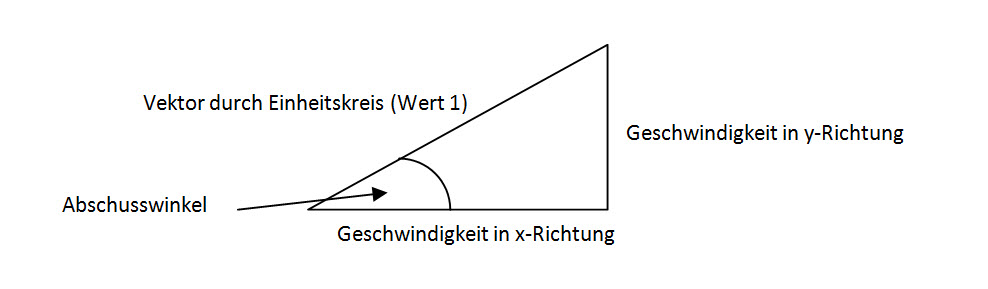
\includegraphics[width=10cm]{Winkel.jpg}
\caption{Berechnung erster Richtungsvektoren}
\end{center}
\label{fig2}
\end{figure} 
So kriegen wir eine anst"andige Ausgangslage, mit der wir auch die Flugbahn besser berechnen k"onnen.
\linebreak

Der Rest der Berechnung l"auft wieder gleich wie beim Satelliten. Die Rakete hat noch die Eigenschaft, dass sobald der Tank leer ist, sie zu einem Satelliten mutiert und dann die Satellitenbeschleunigung alleine gilt.

\newpage

\subsection{Wichtige Codestellen}
\subsubsection{Calculation.java}
\begin{mylisting}
\begin{verbatim}
public double[] diff_mis(double[] yAnfang,double t, Earth earth, Missile missile){
		double[] z = new double[yAnfang.length];
		double[] res = new double[yAnfang.length];
		double[] u = new double[2];
		double uBetrag,vBetrag,m,k,mmissile;

		m = earth.getMass();	// Masse der Erde
		mmissile = missile.getMass() + missile.getTank();
		for(int i=0;i<yAnfang.length;i++)
			z[i] = yAnfang[i];

		u[0] = z[0] - (earth.getPosx() + earth.getRad()/2);
		u[1] = z[1] - (earth.getPosy() + earth.getRad()/2);

		uBetrag = Math.sqrt(u[0]*u[0] + u[1]*u[1]);		//Distanz zwischen Rakete und Erde
		vBetrag = Math.sqrt(z[2]*z[2] + z[3]*z[3]);

		k = 400;											//Leistungskonstante

		//Ableitung von x- und y-Koordinate wird zur Geschwindigkeit
		res[0] = z[2];
		res[1] = z[3];

		//System.out.println(missile.getVx() + ", " + missile.getVy());
		//Ableitung von x- und y-Geschwindigkeit wird zur Beschleunigung
		if (missile.getTank() > 0.0)	{
			res[2] = -g*m*(u[0]/Math.pow(uBetrag, 3)) + (((k*missile.getVerbrennung())/mmissile)*(z[2]/vBetrag));
			res[3] = -g*m*(u[1]/Math.pow(uBetrag, 3)) + (((k*missile.getVerbrennung())/mmissile)*(z[3]/vBetrag));
			missile.setTank(missile.getTank()-(t*missile.getVerbrennung()));
		}
		else {
			res[2] = -g*m*(u[0]/Math.pow(uBetrag, 3));
			res[3] = -g*m*(u[1]/Math.pow(uBetrag, 3));
		}
		return res;
	}
 
	public double[] euler_mis(double tAnfang,double tEnde,double[] yAnfang, int n,Missile missile){
		double h = (tEnde-tAnfang)/n;	//korrektes h f"ur Unterschiede berechnen

		double[] y = yAnfang;
		double[] k;
		double t = tAnfang;

		for(int i=1;i<=n;i++){
			k = diff_mis(y,h,new Earth(),missile); //Ableitung des momentanen Vektors

			y = addVector(y,multScalarVector(h,k));	//neuer Vektor berechnen
			t = t+h;
		}
		return y;
	}
\end{verbatim}
\end{mylisting}

\newpage
\section{L"osungsansatz}
Um das Ziel zu erreichen, dass die abgeschossene Rakete auch den Satellit trifft, stellen wir gewisse "uberlegungen auf. So m"ussen wir wissen, ob die Rakete "uberhaupt die Laufbahn des Satelliten erreichen kann. Wenn wir den Satellit einfach definieren, kann der Fall eintreten, dass die Rakete niemals die Punkte mit der Zielgeschwindigkeit erreicht. So w"are die Aufgabe nat"urlich auch unl"osbar. Um diesem Problem entgegenzuwirken nehmen wir an, dass der Satellit zuvor noch eine Rakete war. Wir schiessen diese in eine Umlaufbahn. Rakete 1 hat also nun ihren Treibstoff verbraucht und ist zu diesem Zeitpunkt zu einem Satellit geworden. So wissen wir nun sicher, dass diese Laufbahn erreichbar ist.
\linebreak

Rakete 1 kreist nun um die Erde. Rakete 2 wird nun mit leicht anderen Werten gef"uttert. Dabei soll nun von alleine ein Wert angepasst werden, damit schlussendlich die Umlaufbahnen "ubereinstimmt.
\linebreak

Das Ganze l"auft also auf folgendes hinaus:
\begin{equation}
Rakete 1
\left(\begin{array}{c}
Pos_{x} \\
Pos_{y} \\
v_{x} 	\\
v_{y}	\\
\end{array}\right)
=
Rakete 2
\left(\begin{array}{c}
Pos_{x} \\
Pos_{y} \\
v_{x} 	\\
v_{y}	\\
\end{array}\right)
\end{equation}
Und das zu einem Zeitpunkt t.
\linebreak

Der Ansatz in der Programmierung ist nun, die Vektoren der Raketen (mit Inhalt Pos\textsubscript{x}, Pos\textsubscript{y}, v\textsubscript{x} und v\textsubscript{y}) von einander zu subtrahieren. Dabei muss als Resultat f"ur jeden einzelnen Vektoreintrag der Wert 0 herauskommen. So k"onnen wir sagen, dass die Raketen mit der gleichen Geschwindigkeit und an der gleichen Position sind. Als Variablen im System sind daher die Treibstoffmenge, der Abschusswinkel, die Zeit zum Treffpunkt gelistet

\newpage

\chapter{Entwicklung}
In diesem Teil betrachten wir prim"ar die Entwicklung. Wir m"ochten diese geradewegs aufteilen auf die 4 Iterationen welche genutzt werden konnten. Zuerst aber werden wir aber unsere Zeitrechnung pro Iteration noch darlegen.
\section{Aufwand pro Iteration}
Vorgabe der Leitung waren 5 Stunden pro Woche. Die Teamgr"osse ist auf 2 Personen begrenzt. F"ur die Fallstudie sind 12 Wochen eingeplant.
\begin{equation}
5\textnormal{ Stunden} * 12\textnormal{ Wochen} * 2\textnormal{ Personen} = 120\textnormal{ Stunden (ohne Abz"uge)}
\end{equation}
Die Velocity setzen wir auf 0.7, da dies ein guter Standard war.
\begin{equation}
120 * 0.7 = 84
\end{equation}
Da wir 4 Iterationen haben brauchen wir f"ur eine Iteration 21 Stunden.
\begin{equation}
\frac{84\textnormal{ Stunden}}{4\textnormal{ Iterationen}} = 21\textnormal{ Stunden}
\end{equation}
Zum Schluss ergeben sich daraus die Stunden pro Person.
\begin{equation}
\frac{21\textnormal{ Stunden}}{2\textnormal{ Personen}} = 10.5\textnormal{ Stunden.}
\end{equation}
\newpage
\subsection{Iteration 1}
\subsubsection{Meilensteine}
GUI erstellt,  Klassendiagramm,  Tasks,  Projektplan, Entwicklungsumgebung
\subsubsection{Ablauf}
Da uns schulischer Stoff noch fehlte um direkt mit der Mathematik zu beginnen, konzentrierten wir uns zuerst auf die Entwicklungsumgebung, die administrativen Arbeiten und das Erstellen der GUI. Wir entschieden uns f"ur die Entwicklung in Java in Verbindung mit Maven und Github. Wir benutzen Maven f"ur ein einheitliches Kompilieren mit externen Java-Libraries. Github wird unsere Versionskontrolle sein, damit wir uns gegenseitig nicht st"oren bei der Entwicklung.
\linebreak

Wir haben uns f"ur diese Tools entschieden, da wir selber nicht als Entwickler arbeiten und uns andere Programme und Sprachen nicht wirklich gel"aufig sind. Im Kurs „Methoden der Programmierung“ haben wir genau diese Tools n"aher angeschaut.
\linebreak

Unser Github ist zu finden unter\linebreak
\href
{https://spitzbueb@github.com/spitzbueb/Inf_Proj.git}%
{www.github.com}
\linebreak

Wir senden unsere "anderungen auf den Server durch folgenden Ablauf:
\begin{itemize}
\item git add .
\item git commit -m 'Beschreibung der "anderung'
\item git push project master (project kann abweichen)
\end{itemize}
F"ur den Download gibt es den Befehl
\begin{itemize}
\item git pull project master
\end{itemize}
So haben wir nun die Speicherumgebung erstellt.
\linebreak

Maven benutzen wir dazu, eine einheitliche Kompilierungsumgebung zu bauen. So erstellen wir zuerst einmal ein Maven-Java-Projekt. Danach bearbeiteten wir die POM.xml und f"ugten unsere gew"unschten Plugins hinzu (wie Javadoc, Testing, usw). Mit „mvn package“ k"onnen wir nun kompilieren lassen und Maven l"adt geradewegs alle Plugins herunter. Unter dem Verzeichnis target wird dann ein ausf"uhrbares JAR-File erstellt.
\linebreak

Unsere n"achsten Ziele waren dann die Tasks (per Scrumy) und der Projektplan. 
In Scrumy haben wir uns die Tasks folgendermassen aufgeteilt:\linebreak
\begin{figure}[H]
\centering
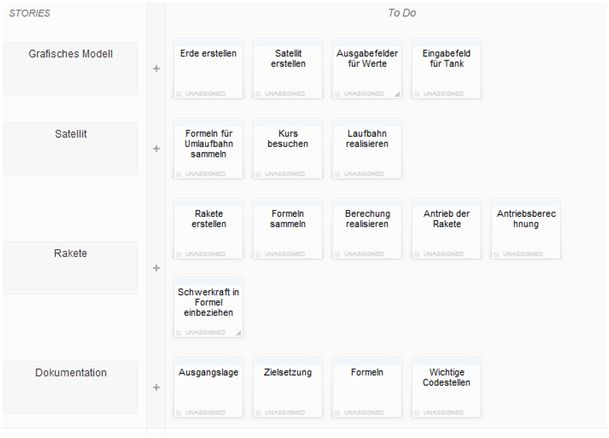
\includegraphics[width=13cm]{Scrumy.jpg}
\caption{Scrumy-Tasks}
\label{fig3}
\end{figure}
\newpage
Aus den Scrumy-Tasks wurde dann der Iterationsplan zusammengestellt.\linebreak
\begin{figure}[H]
\centering
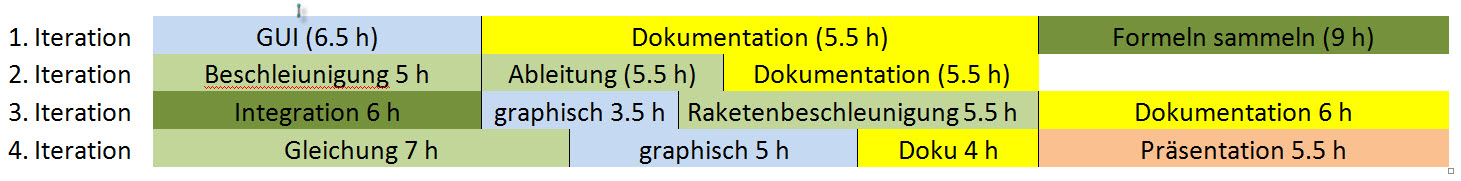
\includegraphics[width=13cm]{Projektplan.jpg}
\caption{Iterationsplan}
\label{fig4}
\end{figure}
Die Planung des Projekts war bis jetzt also erfolgreich. Nun "uberlegten wir uns eine gute M"oglichkeit, wie wir die Klassen zu designen hatten. Ganz getreu der Idee des objekt-orientierten Programmieren Entschieden wir uns f"ur einen Aufbau, der Rakete, Erde, Satellit trennen sollte. So erstellten wir mal die aufgelisteten Klassen:
\begin{itemize}
\item Earth
\item Satellite
\item Missile
\item App
\item Animation
\end{itemize}
\newpage
Nun hatten wir mal unser Grundger"ust. Aber wie sich sp"ater noch herausstellen sollte, mussten wir es doch noch stark erweitern. Aber dies erst in Iteration 2.\linebreak
F"ur das GUI haben wir uns dieses Bild vorgestellt:
\begin{figure}[H]
\centering
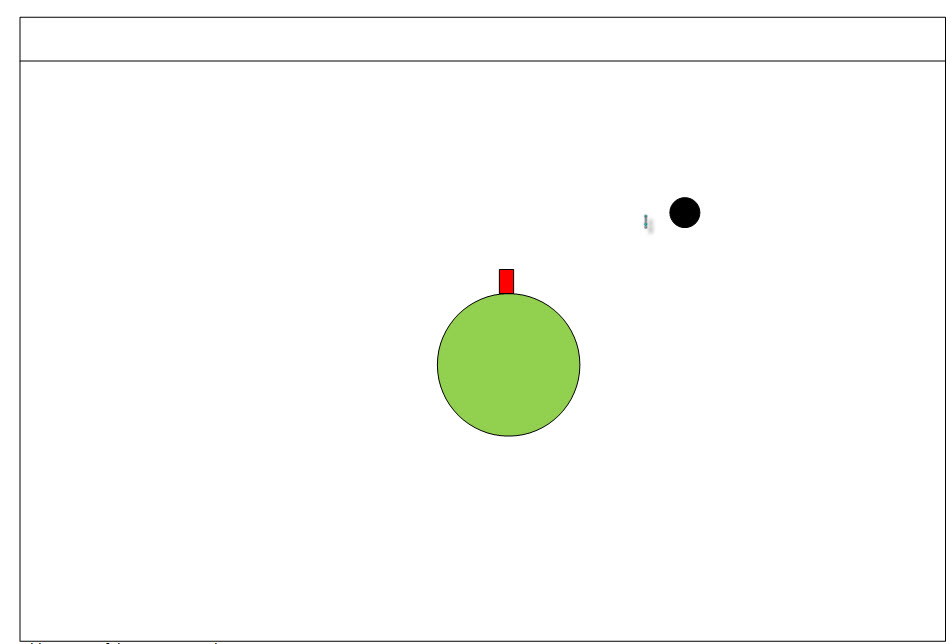
\includegraphics[width=13cm]{GUI.jpg}
\caption{GUI}
\label{fig5}
\end{figure}
Der gr"une Kreis stellt die Erde dar. Der Schwarze den Satelliten und das rote Rechteck die Rakete. Die Men"us werden im oberen Balken untergebracht. Wie diese allerdings aussehen sollten, haben wir uns noch nicht konkret "uberlegt.
\subsubsection{Fazit}
Iteration 1 ist beendet und wir haben unsere Ziele eigentlich alle erreicht. Wir haben allerdings kein Klassendiagramm erstellt. Die Hauptziele, ein GUI sowie die Planung zu haben, sind aber erreicht worden. Die Zusammenarbeit war gut und sollte es so weiter gehen, sollte das Projekt eigentlich keine Umst"ande bereiten.
\subsection{Iteration 2}
\subsubsection{Meilensteine}
Formeln f"ur Berechnung verstehen, Berechnung Satellit und Rakete
\subsubsection{Ablauf}
F"ur die Iteration 2 wollten wir uns komplett auf die mathematischen Teile konzentrieren. Das heisst, in dieser Zeit wurde mehr auf Papier gearbeitet, als Programmcode geschrieben.
Der Start war die Zusatzschulstunde, die Herr Heuberger gegeben hat, damit wir die Berechnung durch Euler schon kennen lernten. Er gab uns noch einige Beispiele wie er funktioniert.
Allerdings mussten wir feststellen, dass uns jegliche Grundlagen in der Physik fehlten um die Flugbahn der zwei Objekte zu berechnen. So waren wir eine bis zwei Wochen damit besch"aftigt, die Formel f"ur die Beschleunigung zu suchen und das Ganze zu verstehen (leider waren die Java-Beispiele schlecht dokumentiert). Wir verabredeten uns mit Herr Heuberger um die Formel des Satelliten nochmals anzuschauen. Er half uns dann, nachdem wir die Situation gekl"art hatten, weiter mit der Formel. Leider konnten wir diese aber nicht bis zum Iterationsmeeting einbauen, was dazu f"uhrte, dass wir nicht wirklich einen Fortschritt pr"asentieren konnten. Erfreulicherweise gelang es aber am darauffolgenden Tag den Satelliten korrekt kreisen zu lassen.
\subsubsection{Fazit}
Es braucht viel Zeit nur schon die Eulerintegration zu verstehen. Dieses Thema wird im Fach Numerik erst gegen Ende des Semesters angeschaut.
Auch die physikalischen Gesetze des Satelliten (und nat"urlich auch der Rakete) waren uns nicht bekannt. Da wir in der ZHAW niemals diese Themen besprochen hatten, hatten wir starke Schwierigkeiten hier weiterzukommen.
Im Meeting mit Herr Heuberger wurde uns aber nochmals alles erkl"art und der Schleier hat sich gel"uftet.
\linebreak

Im Iterationsmeeting hingegen stießen wir f"ur diese Problematik auf taube Ohren. Vielleicht lag es auch daran, dass wir unter Zeitdruck standen, da auch noch Pr"ufung war.
\linebreak

Insgesamt war die Iteration 2 ein kleines Desaster und wir m"ussen nun in der Iteration 3 und 4 diese Fehler sehr schnell korrigieren.
\newpage
\subsection{Iteration 3}
\subsubsection{Meilensteine}
Rakete eingebaut und flugf"ahig, L"osungskonzept begonnen und so gut wie m"oglich umgesetzt, Dokumentation auf aktuellen Stand gebracht
\subsubsection{Ablauf}
Nach dem Desaster aus Iteration 2 mussten wir uns neu organisieren. Der Satellit kreiste nun korrekt um die Erde. Wir hatten also mit einem Tag Versp"atung das Konstrukt bereit. Wir setzten uns nun an die Formel f"ur die Rakete. Gefunden haben wir die Raketengleichung. Allerdings stellte sich heraus, dass diese Formel viel zu kompliziert f"ur unser Vorhaben war.
Herr Heuberger war eine Woche nicht verf"ugbar. In dieser Zeit hatten wir haupts"achlich mit der Rakete gerungen. Die Idee, die Geschwindigkeit in X- und Y-Richtung durch Sinus und Cosinus berechnen zu lassen (da der Abschusswinkel ja eingegeben wird), stellte sich als gute Idee heraus. Nachdem Herr Heuberger wieder zur"uck war, setzten wir uns nochmals zusammen, damit wir die Formel von ihm so absegnen lassen konnten. "uber das folgende Wochenende wurde dann die Rakete fertig implementiert. Auch hatten wir schon die L"osungsidee begonnen einzuf"ugen (2 Raketen, erste wird zum Satellit) um nur noch um das Treffen zu k"ummern.
\linebreak

Probleme gab noch die versetzt startende Animation. Rakete 2 soll ja auf der Erde bleiben, bis sie weiss, wann sie abfliegen muss. 
\subsubsection{Fazit}
Die Ziele der Iteration 3 wurden mehr oder weniger erreicht. Die Rakete war flugf"ahig und ein L"osungskonzept hatten wir auch. Die Dokumentation wurde ebenfalls erweitert. Allerdings sind wir auf die Tatsache gestossen, dass die Pr"asentationstermine (und damit das Ende der Projektzeit) um eine Woche nach vorne geschoben wurde. 
Grunds"atzlich wurden unsere gesteckten Ziele aber erreicht.
\newpage
\subsection{Iteration 4}
\subsubsection{Meilensteine}
Rakete 2 trifft Satellit, Dokumentation beendet, Pr"asentation
\subsubsection{Ablauf}
Wir haben uns f"ur diese Iteration aufgeteilt. Einer konzentriert sich auf die Programmierung des Kollidierens der Raketen. Der andere k"ummert sich um die Dokumentation und die Pr"asentation.
Da die Dokumentation laufend erweitert wurde, haben wir hier nicht so einen grossen Klotz am Bein. Allerdings m"ussen wir die Pr"asentation noch erstellen.
Das Treffen der beiden Flugk"orper hingegen bereitet noch weiter Schwierigkeiten. Vor allem die "uberlegung, dass die Rakete auch in die gleiche Flugbahn geraten soll. Wenn der Abschusswinkel und die Tankf"ullung verschieden zur ersten Rakete sind, dann wird die zweite Rakete nie in die gleiche Umlaufbahn kommen, ohne noch Steuerungselemente zu besitzen. Sie k"onnen also nur kollidieren.

\subsubsection{Fazit}
Das Projekt ging nun in die letzte Phase ein. Die Aufteilung war eine gute Idee, und so konnte die Dokumentation zum Beispiel von einem Word-Dokument noch in ein LaTeX-Dokument konvertiert werden. Die Pr"asentation findet am 15.06.2012 statt. Wir werden sehen, wie unsere L"osung ankommen wird.
\newpage
\chapter{Resultat, Fazit und Danksagung}
\section{Resultat}
Am Beispiel des Satelliten m"ochten wir zuerst zeigen, dass wirklich eine elliptische Bahn entsteht mit unserer Formel. Da die Rakete nach dem Start sich in einen Satelliten verwandelt, gilt diese Beziehung auch f"ur diese. Allerdings wird die entsprechende Flugbahn anders verlaufen. Als Beispiel nehmen wir einen Satelliten, welcher schon in der Umlaufbahn ist. Er hat die Positionskoordinaten (0/60) f"ur X und Y und den Geschwindigkeitsvektor (50/20). Die Flugbahn soll von t\textsubscript{0} bis t\textsubscript{ende} = 80 berechnet werden.
\linebreak

\begin{tabular}{ccccc}
t & Pos\textsubscript{x} & Pos\textsubscript{y} & v\textsubscript{x} & v\textsubscript{y} \\
0 & 0 & 60 & 50 & 20 \\
1 & 87.922 & 65.832 & 36.645 & -6.683 \\
2 & 150.101 & 46.087 & 26.451 & -11.865 \\
3 & 196.289 & 20.776 & 20.175 & -13.148 \\
4 & 232.068 & -5.799 & 15.834 & -13.323  \\
5 & 260.334 & -32.246 & 12.569 & -13.081 \\
6 & 282.784 & -58.001 & 9.969 & -12.654 \\
7 & 300.504 & -82.801 & 7.812 & -12.136 \\
8 & 314.238 & -106.512 & 5.966 & -11.569 \\
9 & 324.521 & -129.059 & 4.349 & -10.974 \\
10 & 331.748 & -150.394 & 2.904 & -10.359
\end{tabular}
\linebreak

Die Werte sind auf 3 Nachkommastellen gek"urzt. Dieser kurze Ausschnitt soll die Entwicklung zeigen. Wenn wir nun die Tabelle fortf"uhren bis t = 40, werden wir eine elliptische Bahn bekommen. Diese sehen wir, sobald die X- und Y-Koordinaten plotten.
\linebreak
\begin{figure}[H]
\centering
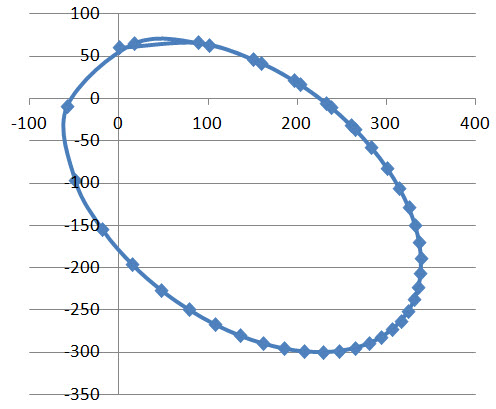
\includegraphics[width=13cm]{elliptische_bahn.jpg}
\caption{elliptische Bahn des Satelliten durch Euler-Integration}
\label{fig6}
\end{figure}
\section{Fazit}
Die Thematik des Projekts war sehr interessant. Die Motivation, das komplexe Thema zu schaffen war hoch. Leider untersch"atzten wir die komplette Berechnung des Systems. So verloren wir viel Zeit w"ahrend der zweiten Iteration. Die Theorie von Euler war f"ur uns sehr abstrakt und am Anfang schwer zu verstehen. Die Programmierung des kreisenden Satelliten (und sp"ater der fliegenden Raketen) hingegen war schon eher leicht. Daher konnten wir in der Iteration 3 Zeit wett machen und unser Projekt auf Vordermann bringen. \linebreak
Die letzte Iteration lag (wie schon erw"ahnt) komplett in den H"anden der Dokumentation und der Pr"asentation. \linebreak
Schlussendlich kommen wir darauf, dass das Projekt sehr interessant war, uns einiges beigebracht hat was Mathematik an einem geschlossenem System, Planung und Realisierung eines Projekts und verschiedenen Tools angeht. Leider haben wir auch erfahren m"ussen, dass eine Leitung nicht immer wirklich gut leitet. Informationen wurden nicht weitergegeben und Meetings sehr kurzfristig und zu unm"oglichen Zeiten angesetzt. Dies nur als Beispiel. Trotzdem war es toll, das gelernte mal gut, mal weniger gut anzuwenden.
\section{Danksagung}
An dieser Stelle m"ochten wir Herr Albert Heuberger danken. Er hat uns w"ahrend der Projektarbeit tatkr"aftig unterst"utzt. Er war auch ausserhalb der Schulzeit bereit, mit uns mathematische Probleme anzuschauen und m"ogliche L"osungskonzepte aufzuzeigen. Besonders zu erw"ahnen w"are der zus"atzliche Samstag, welchen er den „Projektlern“ angeboten hat. Dort gab er uns die Chance, numerische Themen schon im Voraus  zu betrachten, da diese erst gegen Ende Semester Teil des Stoffplanes waren. So konnten wir die M"oglichkeiten gut aussch"opfen.
\begin{thebibliography}{100}
\bibitem{Hallyday} David Halliday, Robert Resnick, Jearl Walker; Halliday Physik Bachelor-Edition ; Verlag Wiley-VCH; ISBN 978-3-527-40746-0
\bibitem{grafik} Grafiken zeichnen in SWING \linebreak \href{http://www.javabeginners.de/Grafik/geometrische_Grundformen_zeichnen.php}
{www.javabeginners.de} \linebreak Abrufdatum: 25. M"arz 2012
\bibitem{maven} Maven Installation, Dokumentation \linebreak \href{http://maven.apache.org}{maven.apache.org} \linebreak Abrufdatum: 19. M"arz 2012
\bibitem{git} Git Dokumentation \linebreak
\href{http://www.github.com}{www.github.com} \linebreak Abrufdatum: laufend (lezte 30.Mai.2012)
\bibitem{wiki} Wikipedia \linebreak
\href{http://www.wikipedia.org}{www.wikipedia.org}
\linebreak Abrufdatum: 26. April 2012
\end{thebibliography}
\end{document}